% Lancaster Data Science Hackathon — Beamer slides
% -----------------------------------------------------------------------------
% Build with `make` (uses XeLaTeX via latexmk).  Edit the metadata block below
% and add frames between \begin{document} / \end{document}.
% -----------------------------------------------------------------------------

\documentclass[aspectratio=169,11pt]{beamer}

% --- Theme -------------------------------------------------------------------
\usetheme[progressbar=frametitle, numbering=fraction,
          sectionpage=progressbar, subsectionpage=progressbar]{metropolis}

\usepackage{booktabs}
\usepackage{graphicx}
\usepackage{amsmath}
\usepackage{xcolor}
\usepackage{hyperref}
\usepackage{href-ul}

% --- Code snippets -----------------------------------------------------------
% `listings` is the default: robust, no shell-escape needed.  A `minted`-based
% alternative (needs `pygmentize` + -shell-escape, already enabled in the
% Makefile) is shown commented out below.
\usepackage{listings}

\definecolor{codebg}{HTML}{F5F5F5}
\definecolor{codekw}{HTML}{1F4E79}
\definecolor{codestr}{HTML}{8A6A1F}
\definecolor{codecom}{HTML}{6A737D}

\lstdefinestyle{slidecode}{%
  basicstyle      = \ttfamily\footnotesize,
  backgroundcolor = \color{codebg},
  keywordstyle    = \color{codekw}\bfseries,
  stringstyle     = \color{codestr},
  commentstyle    = \color{codecom}\itshape,
  showstringspaces= false,
  breaklines      = true,
  frame           = none,
  xleftmargin     = 0.5em,
  xrightmargin    = 0.5em,
  aboveskip       = 0.8em,
  belowskip       = 0.6em,
  literate        = {->}{{$\rightarrow$}}1,
}
\lstset{style=slidecode}

% `listings` has no built-in TOML language, so define a minimal one.
\lstdefinelanguage{TOML}{
  keywords      = {true, false, inf, nan},
  morecomment   = [l]{\#},
  morestring    = [b]",
  morestring    = [b]',
  alsoletter    = \{-\},
  sensitive     = true,
}

% --- minted alternative (uncomment to use; requires pygmentize) -------------
% \usepackage{minted}
% \usemintedstyle{friendly}
% \setminted{fontsize=\footnotesize, breaklines, bgcolor=codebg, frame=none}
% \newcommand{\inputmintedfile}[2]{\inputminted{#1}{#2}}

% Helper for inline code / file paths / identifiers in prose.
\newcommand{\code}[1]{\texttt{#1}}

% --- Metadata ----------------------------------------------------------------
\title{Lancaster Data Science Hackathon}
\subtitle{Data Analysis in Python}
\author{Clio Johnson}
\institute{School of Mathematical Sciences, Lancaster University}
\date{26${}^\text{th}$ of November, 2026}

\begin{document}

\maketitle

\begin{frame}{Outline}
  \tableofcontents
\end{frame}

\section{Introduction}

\begin{frame}{Welcome to the Hackathon}
  The goal today is to discover and present some interesting results from one of three datasets.
  \vspace{12pt}
  \begin{columns}[t]
    \begin{column}{.333\textwidth}
      Energy Usage data at Lancaster University.
    \end{column}
    \begin{column}{.333\textwidth}
      Radar signals from various human activities.
    \end{column}
    \begin{column}{.333\textwidth}
      Genes present in tiny slices of a mouse brain.
    \end{column}
  \end{columns}
  \vspace{12pt}
  This talk will introduce those datasets and serve as a quick tutorial on how to interact with them in Python.
\end{frame}

\begin{frame}[fragile]{Python Setup}
    To get you started, I have made a template repository on Github: \href{https://github.com/muse-writes/lancaster-data-science-hackathon}{muse-writes/lancaster-data-science-hackathon}\\
    \vspace{12pt}
    Please clone it in your IDE of choice, or using:
    \begin{lstlisting}[language=Bash]
$ git clone <git-url> lancaster-data-science-hackathon/
    \end{lstlisting}
    \begin{columns}[T]
      \begin{column}{.45\textwidth}
        \raggedleft
        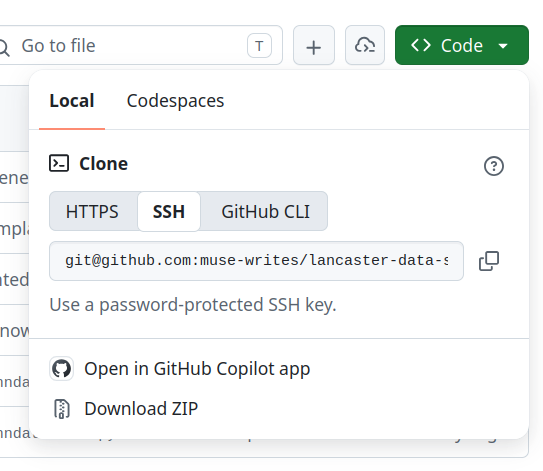
\includegraphics[width=0.7\linewidth]{images/git-url.png}
      \end{column}
      \begin{column}{.45\textwidth}
        \vspace{48pt}
        $\leftarrow$ Obtain the \texttt{<git-url>} from here.
      \end{column}
    \end{columns}
\end{frame}

\section{Data}

\begin{frame}{Available datasets}
  Today's datasets are available from a shared OneDrive directory:
  \begin{center}
  \begin{tabular}{ll}
    \toprule \midrule
    Dataset & Description \\
    \midrule
    Energy Usage & 10-min kWh consumption for 5 campus buildings \\
    RadarData    & Micro-Doppler spectrograms of common human activities \\
    Mouse Brain  & Mouse brain transcriptomics pucks.\\
    \midrule \bottomrule
  \end{tabular}
  \end{center}
\end{frame}

\begin{frame}{Data setup}
  To use each of the datasets with the template repository.
  \begin{itemize}
    \item Download them from the OneDrive.
    \item Make a \texttt{./data} folder in your template repository.
    \item Extract the zipped folders into \texttt{./data}.
  \end{itemize}
  The utilities provided in \texttt{src} for loading the data use these locations as defaults.
\end{frame}

\begin{frame}[fragile]{Data setup}
  Your file structure should look something like this:
  \begin{lstlisting}[language=Bash]
path/to/lancaster-data-science-hackathon/
-----------------------------------------
.git/
.pixi/
data/
 | 'Energy Usage'/
 | 'Mouse Brain'/
 | RadarData/
slides/
src/
.gitattributes
.gitignore
README.md
pixi.lock
pyproject.toml
  \end{lstlisting}
\end{frame}

\section{Python Libraries}

\begin{frame}[fragile]{Package Overview}
  The previous slide introduced the package structure. We're going to use \href{https://pixi.prefix.dev/latest/#installation}{\texttt{pixi}} to manage dependencies for convenience.
  \begin{figure}
    \centering
    
\includegraphics[width=0.3\linewidth]{images/pixi.png}
    \caption{Pixi manages your virtual environment.}
  \end{figure}
\end{frame}

\begin{frame}[fragile]{\texttt{pyproject.toml}}
  Open the file named \texttt{pyproject.toml} in a text editor. This is where Python packages are configured. You will see some basic metadata:
  \begin{lstlisting}[language=TOML]
[project]
authors = [{name = "Clio Johnson", email = "d.k.johnson@lancaster.ac.uk"}]
dependencies = []
name = "lancaster-data-science-hackathon"
requires-python = ">= 3.11"
version = "0.1.0"
  \end{lstlisting}
  \vspace{12pt}
  Edit the name and email so that it points to yourself!
\end{frame}

\begin{frame}[fragile]{\texttt{pyproject.toml} (contd.)}
  Scrolling down, you will see the list of dependencies that \texttt{pixi} will install
  \begin{lstlisting}[language=TOML]
[tool.pixi.dependencies]
pandas = ">=3.1.0,<4"
numpy = ">=2.5.4,<3"
scipy = ">=1.18.1,<2"
ruff = ">=0.17.6,<0.18"
ipython = ">=9.18.1,<10"
anndata = ">=0.11"
  \end{lstlisting}
  \vspace{12pt}
  You might be wondering why there's no \texttt{matplotlib}\ldots
\end{frame}

\begin{frame}[fragile]{Managing a project with Pixi}
  In your command line, pixi lets you reproducibly install the provided environment:
  \begin{lstlisting}[language=Bash]
$ pixi install
  \end{lstlisting}
  and then add new dependencies with
  \begin{lstlisting}[language=Bash]
$ pixi add matplotlib
  \end{lstlisting}
\end{frame}

\begin{frame}{Data Analysis in Python}
  The provided environment contains several packages you may want to use for data analysis, and some which are required for certain datasets in this hackathon.
  \vspace{6pt}
  \begin{center}
    \begin{tabular}{lll}
      \toprule
      Package & Purpose & Required for \\
      \midrule
      \texttt{pandas}  & Tabular data             & Energy Data \\
      \texttt{numpy}   & Numerical arrays         & Radar Data \\
      \texttt{scipy}   & Scientific computing     & Radar Data \\
      \texttt{anndata} & Annotated matrices       & Mouse Brain \\
      \texttt{ipython} & Interactive Python shell & --- \\
      \bottomrule
    \end{tabular}
    \end{center}
  \vspace{6pt}
\end{frame}

\begin{frame}[fragile]{\texttt{numpy}}
  So, let's cover some basics: \texttt{numpy} is a library providing very well optimised numerical arrays and functions which act upon them. \\
  The \texttt{ndarray} is an array of numerical values which are all of the same type. Import and create an array using
  \begin{lstlisting}[language=Python]
import numpy as np
my_array = np.array([1., 2., 3.], dtype=np.float64)
  \end{lstlisting}
  Python loops are slow, so use \texttt{numpy}'s compiled element-wise or vectorised functions.
  \begin{lstlisting}[language=Python]
a * b               # Elementwise multiplication.
A @ B               # Matrix multiplication.
np.sqrt(my_array)   # Elementwise square-root operation.
  \end{lstlisting}
  Linear algebra functions can be found in the module \texttt{np.linalg}
\end{frame}

\begin{frame}[fragile]{\texttt{numpy} (contd.)}
  For statistics you may find the following numpy functions useful:
  \begin{lstlisting}[language=Python]
a.sum()             # Sum of a list's elements.
a.mean(), a.std()   # Mean and standard deviation.
a.min(), a.max(), a.argmin(), a.argmax()
  \end{lstlisting}
  As well as the usual Python array slicing behaviour. You can apply boolean masks to grab a subset of some data, for instance:
  \begin{lstlisting}[language=Python]
a = np.load("a.npy")
mask = a > 0.
a_gt_zero = a[mask]
  \end{lstlisting}
\end{frame}

\begin{frame}[fragile]{\texttt{numpy} (contd.)}
  Prepare histogram data with
  \begin{lstlisting}[language=Python]
counts, edges = np.histogram(a, bins=30, density=True) # density = histogram integrates to 1.
  \end{lstlisting}
\end{frame}

\begin{frame}[fragile]{\texttt{scipy}}
  \texttt{scipy} is a large collection of scientific computing routines, organised into submodules:
  \texttt{stats}, \texttt{linalg}, \texttt{optimize}, \texttt{signal},
  \texttt{fft}, \texttt{sparse}, and \texttt{io}. Import the submodule you need:
  \begin{lstlisting}[language=Python]
from scipy import stats, linalg, optimize, signal, io
  \end{lstlisting}
  For the radar dataset, \texttt{scipy.io.loadmat()} reads the MATLAB \texttt{.mat} files. \\
\end{frame}

\begin{frame}[fragile]{\texttt{scipy} (contd.)}
    \texttt{scipy.optimize} contains utilities for minimising a loss function (\texttt{scipy.optimize.minimize}) and fitting curves to data.
    \begin{lstlisting}[language=Python]
from scipy.optimize import curve_fit
# Define a simple exponential model with free parameters: a, b, and c.
def model(x, a, b, c) -> np.float64:
    return a * np.exp(-b * x) + c
# Fit the curve using available data, and initial params p0.
params, cov = curve_fit(model, xdata, ydata, p0=[1, 0.1, 0])
    \end{lstlisting}
\end{frame}

\begin{frame}[fragile]{\texttt{scipy} (contd.)}
  \texttt{scipy.stats} provides probability distributions for hypothesis tests etc.
  Each distribution is an object with \texttt{pdf}, \texttt{cdf}, \texttt{ppf}
  and a \texttt{fit} method:
  \begin{lstlisting}[language=Python]
from scipy import stats
# Create a normal distribution N(0, 1)
n = stats.norm(loc=0, scale=1)
n.pdf(0.)     # Calculates the density at 0.
n.cdf(0.)     # Similar with cumulative density.
samples = n.rvs(size=3) # Draw random samples.
  \end{lstlisting}
\end{frame}

\begin{frame}[fragile]{\texttt{pandas}}
  \texttt{pandas} is a library for handling tabular data, stored in \texttt{DataFrame} objects (essentially spreadsheets with named columns and a typed index). Today's energy data loads as a \texttt{dict} of \texttt{pandas} objects.
  \begin{lstlisting}[language=Python]
import pandas as pd
# Read a DataFrame object from a CSV file.
df = pd.read_csv("data/Energy Usage/Data/Library.csv",
                 parse_dates=["time"], index_col="time")
df.head()       # First rows.
df.columns      # Column labels.
df.shape        # (rows, cols)
df.index        # The row index.
  \end{lstlisting}
\end{frame}

\begin{frame}[fragile]{\texttt{pandas} (contd.)}
  Select columns or rows, and summarise with \texttt{groupby}:
  \begin{lstlisting}[language=Python]
df["value"]                 # one column (a Series)
df.loc["2024-01":"2024-03"]  # slice rows by index label
df["value"].resample("D").sum()           # daily totals
df.groupby(df.index.hour)["value"].mean() # mean by hour of day
  \end{lstlisting}
  The energy data in this hackathon has a \texttt{DatetimeIndex}, \texttt{resample} and time-based dataframe slicing work out of the box.
\end{frame}

\begin{frame}[fragile]{\texttt{anndata}}
  \texttt{anndata} provides an \texttt{AnnData} object for annotated 2D matrices. Bundling a raw matrix and some metadata together.
  \begin{lstlisting}[language=Python]
import anndata as ad
# We will be loading this data from H5AD files, a genomics file format.
data = ad.read_h5ad("path/to/data.h5ad")
# Access useful variables with:
shape = data.shape
row_labels, gene_names = data.obs_names, data.var_names
  \end{lstlisting}
    You can also grab the raw matrix itself as \texttt{data.X}, but be careful, it's often \textit{huge} and \textit{sparse} so it's best to work with small slices at once.
\end{frame}

\begin{frame}[fragile]{Loading the data}
  This repository template contains a series of modules and import functions for loading the included data, each returning a \texttt{dict} keyed by an identifier. Their type signatures show which library you should use for each one:
  \begin{lstlisting}[language=Python]
from lancaster_data_science_hackathon import (
    load_energy_data,      # -> dict[str, pd.DataFrame] (pandas)
    load_radar_data,       # -> dict[int, np.NDArray]   (numpy)
    load_mouse_brain_data, # -> dict[int, ad.AnnData]   (anndata)
)
# Defaults to loading from ./data/ # Key            : Data
energy = load_energy_data()        # building name  : DataFrame
radar  = load_radar_data()         # activity class : spectrogram
brain  = load_mouse_brain_data()   # puck number    : AnnData
  \end{lstlisting}
\end{frame}

\begin{frame}[standout]
  Thanks!\\[1ex]
  \small Questions? \\ 
  \vspace{24pt}
  This PDF is available at \texttt{./slides/main.pdf}
\end{frame}

\end{document}
